\documentclass[11pt]{article} % For LaTeX2e
\usepackage{manuscript, palatino}
\usepackage{graphicx}
\usepackage{amsfonts, amsmath}
\usepackage{algorithm, algpseudocode}%

\usepackage{natbib}

\title{Title Pending}

\author{
Samuel Zorowitz \\
Princeton Neuroscience Institute\\
Princeton University\\
Princeton, NJ 08540 \\
\texttt{zorowitz@princeton.edu} \\
\And
Ida Momennejad \\
Columbia University\\
New York, NY 10027 \\
\texttt{ida.m@columbia.edu} \\
\And
Nathaniel Daw \\
Princeton Neuroscience Institute\\
Princeton University\\
Princeton, NJ 08540 \\
\texttt{ndaw@princeton.edu} \\
}

\newcommand{\fix}{\marginpar{FIX}}
\newcommand{\new}{\marginpar{NEW}}

\begin{document}

\maketitle

\begin{abstract}
Pending
\end{abstract}

\keywords{
anxiety; avoidance; fear generalization; decision theory; computational psychiatry
}

\startmain

\section{Introduction}

Anxiety disorders are characterized by aberrations in the cognitive processing of and response to threat. The hallmark symptom of anxiety disorders is exaggerated threat appraisal, or the tendency to perceive threat as disproportionately greater in likelihood and/or severity than is warranted. Clinical anxiety often also involves the generalization of fear, wherein an individual comes to perceive as threatening cues or situations secondarily associated with the primary fear. For example, a dog phobic individual may first fear dog parks, then parks in general, and finally any public space where a dog may plausibly be encountered. Unsurprisingly then, anxiety disorders involve persistent avoidance behavior. Avoidance behaviors in anxiety are especially pernicious as they prevent potential exposure to disconfirming evidence about perceived threats, thereby maintaining the disorder, and because they are often highly disruptive to everyday functioning. Avoidance of perceived threat often comes at considerable expense, either in foregone rewards or in the expenditure of effort. On their walk to work, the same dog phobic individual may take increasingly circuitous paths in order to avoid certain public spaces and may abandon social obligations for fear of encountering a dog. These behaviors are puzzling to theories of learning and choice behavior, not in the least because they are still observed even in safe situations posing little to no objective threat.

Some insight into anxious cognition might possibly be gleaned from a decision theoretic perspective. In decision theory, the value of potential actions (e.g. to approach or avoid) is defined in part as a function of expectations about the future. The best action is that which yields the greatest cumulative reward, contingent on current beliefs of what will likely be encountered in the future. Interestingly, anxiety disorders are associated with pessimistic beliefs about the future; anxious individuals are more likely to endorse beliefs like that they will surely face danger in the future and be unable to respond effectively to it. Despite this common finding, most studies of anxious decision making interrogate behavior in response to immediate but not future threat. Studying anxious appraisal of future threat may be more important for understanding anxiety disorders as symptoms like fear generalization and avoidance show worry for would-be but not immediate danger.

Here, we explore these issues by offering a decision theoretic account of sequential choice under pessimistic future expectations. We consider optimal behavior in deterministic, finite Markov decision processes (MDP), in which agents learn reward-maximizing (or loss-minimizing) policies in grid world environments requiring a series of choices. We first describe a fundamental asymmetry in the differential influence of reward and danger on value estimation under normative models of learning, namely that reward propagates recursively but danger does not. We then demonstrate how this asymmetry is eliminated when agents instead learn with anxious-like expectations of future action. We find that a minor deviation from normativity captures many features of anxious behavior including exaggerated threat appraisals, fear generalization, and persistent avoidance.

In the remaining sections, we also show that this simple model can account for a number of findings reported in the minority of studies that have probed anxious behavior in sequential choice environments. We then offer a novel prediction based on the the model that, consistent with negative future expectations, anxious individuals should not exhibit a free choice premium. We then close with a discussion of the relationship of our decision theoretic account to prominent clinical theories of anxiety, potential extensions to the model, and possible neural correlates.

\section{The model}

We first briefly review the formalism of Markov decision processes, which will provide the framework for our results. For complete treatments, see \cite{SuttonBarto2018} and \cite{bertsekas2005}.

A MDP is defined by a set of states, $S$, a set of actions, $A$, a reward function defined over state-action pairs, $R(s,a)$, and a state transition distribution, $P(s'|s,a)$. In a MDP, states and rewards are experienced sequentially according to chosen actions and the one-step transition structure. The goal for an agent in a MDP is to learn a policy, or mapping of actions to states, that maximizes expected cumulative (discounted) reward. The value of a state can be defined recursively as the sum of the immediate reward received following an action, $R(s, a)$, and the value of its successor state $s’$, averaged over potential future transitions and actions according to the current policy $\pi$. Under Bellman optimality, the value of a state under the optimal policy is equal to the expected return for the best action from that state.

$$ V^*(s) = \max_a \sum_{s',r} p(s',r|s,a) \left[ r + \gamma v(s') \right] $$

where $\gamma$ is the temporal discounting parameter, which controls the influence of distant future rewards.

Crucially then, the value of a state under the optimal policy is contingent on an agent's particular expectations about the future. First, it is a function of the state transition distribution, or beliefs about the likelihood of encountering particular successor states conditioned on performing some action. Second, it is also a function of the actions available in those successor states, as future actions in turn define their value. Under Bellman optimality, it is normative for an agent to assume that the value of a successor state is equivalent to the best action from that state. This can be expressed as:

$$ V^*(s) = \max_a \sum_{s',r}p(s',r|s,a) \left[ r + \gamma \max_{a'} q_*(s',a') \right] $$

where $q(s',a')$ denotes the a state-action value. As we will demonstrate, this assumption has profound consequences for learning about reward and danger.

In a MDP, the discovery of a rewarding action by an agent has an effect not only on the associated state but also on its antecedent states. This follows naturally from the recursive definition of state values defined above. When an agent learns a particular state predicts reward, the states which immediately precede it also acquire value (as do their antecedent states, and so on). The discovery of a rewarding action thus propagates positive value across the state space, so as to motivate the future visitation of rewarding states. A similar spread of value does not occur, however, upon the discovery of a suboptimal or harmful action. Under the optimal policy, only the best action is chosen; a reward-maximizing agent will avoid performing a harmful action insofar that another option is available. When avoidance is possible, the discovery of a harmful action will not impact the value of its associated state. Moreover, an avoidable harmful action will not influence the value of its antecedent states, as is reflected by the max operator in the equation above. Thus, the optimistic assumptions about future behavior under Bellman optimality yields a fundamental asymmetry in the treatment of reward and danger: whereas rewarding opportunity propagates recursively to antecedent states, danger does not whenever avoidance is possible.

This principle is highlight in a toy MDP, the open field environment (Figure 1a). The open field is a grid world that entirely empty except for two states, one rewarding and one harmful. Importantly, the open field MDP is deterministic, such that the one-step transition distribution respects the agent's choice. An agent in this environment then will only experience an aversive outcome if it chooses to approach the dangerous state. The state value estimates learned by an agent under Bellman optimality reflect the asymmetry described above (Figure 1b). In the open field, reward propagates recursively from the source to antecedent states whereas danger does not. Thus the agent learns to associate all states (except the harmful state itself) with positive value. Because harm is avoidable in this environment, all states (even those proximal to threat) come to represent the opportunity for reward.

What happens then when an agent believes (falsely) that danger is not avoidable? In the MDP formalism, such an errant belief may manifest in numerous ways. First, an agent may possess inaccurate assumptions about the state transition distribution. For example, an agent may wrongly believe it possible that it could transition to a state closer to danger in spite of an avoidance action. Alternately, an agent may operate under pessimistic expectations about the availability of future actions. It may believe it has the capacity to act in accordance with the optimal (reward-maximizing) policy in the present, but may be unable to do so in the future. We note here that similar beliefs about the unreliability of self or the environment in the presence of perceived threat are often endorsed in anxiety disorders.

We can easily model pessimistic expectations about future action through a minor change to the definition of state value. Previously introduced by \cite{Gaskett2003}, we define pessimistic learning as the expectation of future deviation from the optimal policy such that the value of a successor state is equal to:

$$ V(s') = w \max_{a'} q(s',a') + (1 - w) \min_{a'} q(s',a') $$

such that the state value under the optimal policy is defined as:

$$ V(s) = \max_a \sum_{s',r}p(s',r|s,a) \left[ r + \gamma \left( w \max_{a'} q(s',a') + (1 - w) \min_{a'} q(s',a') \right) \right] $$

Here, the parameter $w$ controls the degree of pessimism. When $\w = 1$, an agent is maximally optimistic and fully expects to act according to the best possible actions in the future. When $w = 0$, the agent is maximally pessimistic and fully expects to act according to the worst possible actions in the future. When $w = 0.5$, the weighs the best and worst possible future actions equally. We note we are not committed to this particular implementation. Pessimistic learning could be introduced through a variety of other manipulations. We have selected this particular formalism because out of convenience; it does not constitute a mechanistic claim about anxious cognition.

\begin{figure}
  \centerline{%
    \resizebox{1.0\textwidth}{!}{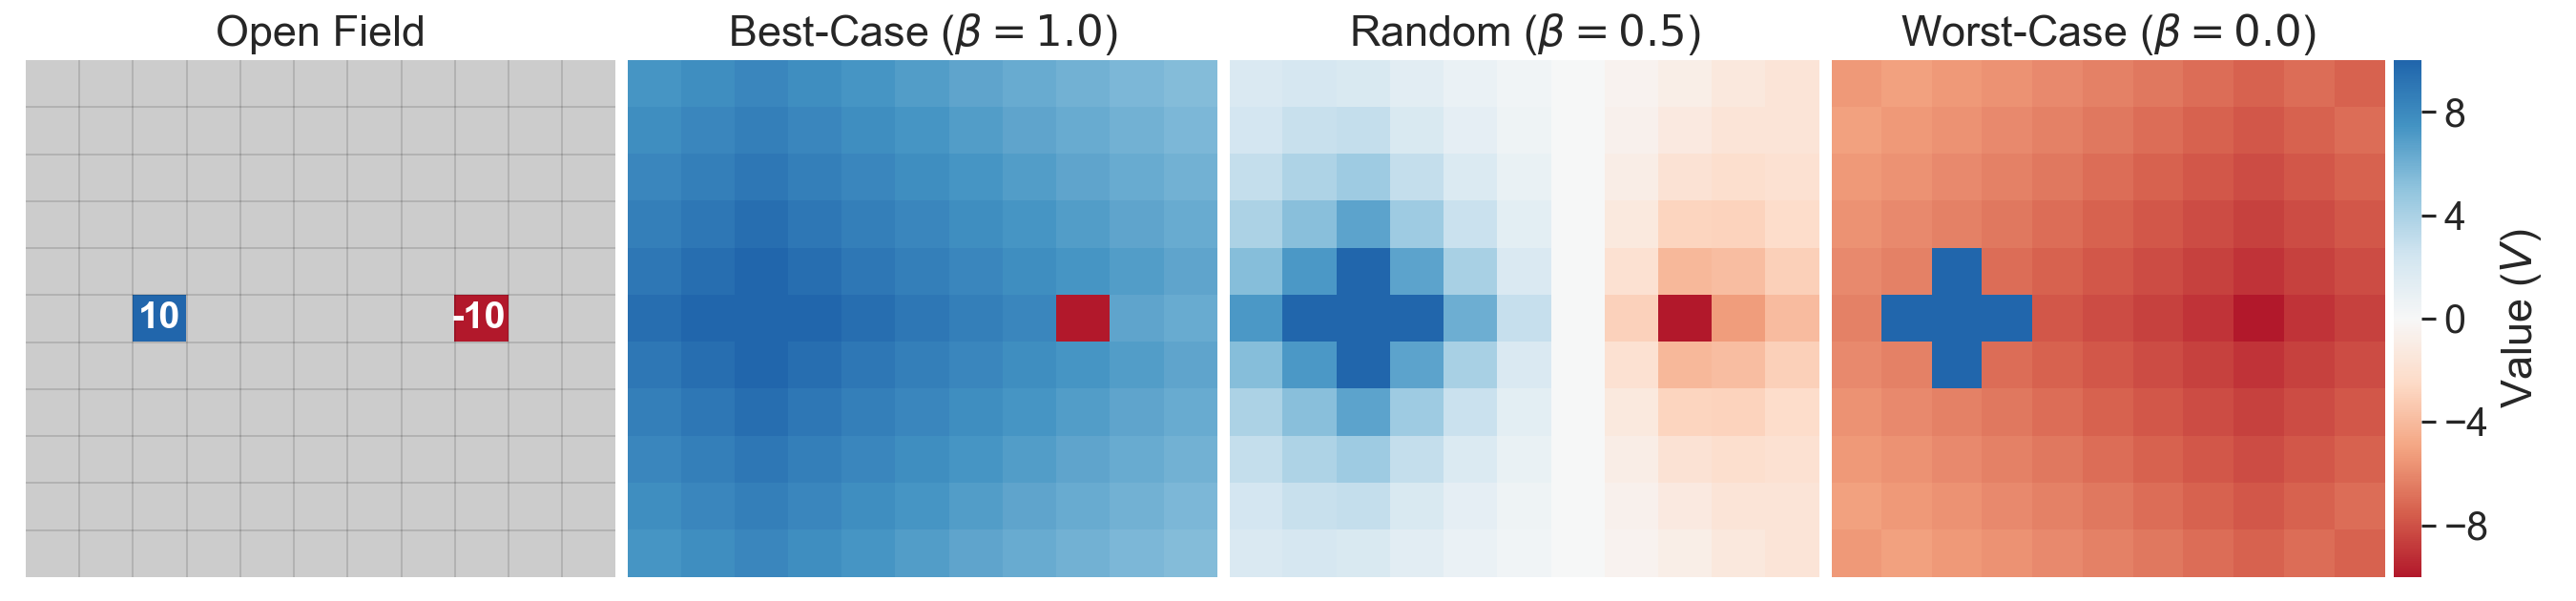
\includegraphics[trim={0 0 0 0},clip]{../figures/01_field.png}}%
  }
  \par \textbf{Figure 1:} The open field is a deterministic gridworld with only one rewarding (blue) and aversive (red) state (A). For an optimistic agent ($w=1$), all states (other than the harmful state) take on positive value (B). For a pessimistic agent ($w=0.5$), negative value spreads from the source to antecedent states (C). With increasing pessimism ($w=0$), the extent of the spread grows worse (D). (Parameters: $\gamma = 0.95$)
\end{figure}

For a pessimistic agent ($w > 0$), the expectation that future action will always be optimal (reward-maximizing) is violated; instead, the agent believes that it may act with some probability in direct contrast to its preferences. Under these conditions, an agent cannot expect to invariably avoid choosing a harmful action. Therefore, the presence of danger now poses threat and safety cannot be guaranteed. The consequences of this manipulation for the open field environment are presented in Figure 1c,d. The deviation from Bellman optimality, wherein the value of antecedent states are contingent on both the best and worst possible future actions, means that now more than reward opportunities are able to propagate recursively through state space. Indeed when $w$ is non-zero, threat value from danger also recursively propagates from its source through adjacent states. The extent of this spread is contingent on the degree of pessimistic belief. As an agent grows increasingly certain of future deleterious action (i.e. $w \rightarrow 1$), the greater the extent to which threat value permeates the state space.

We also note that this simple demonstration produces behaviors similar to the core symptoms of anxiety disorders. As is evidence in Figure 1c,d, the pessimistic agent exhibits exaggerated threat appraisals. It estimates danger at disproportionately more states than is warranted (likelihood bias) and perceives those states as more threatening than they objectively are (severity bias). Similarly, the propagation of threat value is reminiscent of the fear generalization observed in clinical anxiety. Through pessimistic learning the agent comes to regard as threatening states with increasingly distant associations to the danger source.

The model also predicts persistent avoidance behaviors similar to those observed in clinical anxiety. Importantly, the avoidance behavior exhibited by the model begins early in the chain of sequential choices. In other words, the agent performs avoidance before it is proximal to danger. This is because agents in this model act in response to anticipated future threat. Specifically, the agent cannot be certain it will not act against its preferences in the future. To minimize the likelihood of inadvertently encountering danger, the agent therefore places as much distance between itself and the possible danger through early avoidance actions. As discussed in the introduction, this is what is observed both clinically and empirically in studies of anxious individuals responding to threat \citep{Bach2014, Bach2017, Sheynin2014}. Thus our model not only predicts persistent avoidance behavior, but also captures the excessive, overly cautious profile of avoidance behavior exhibited in clinical anxiety.

\section{Simulations}

In the following sections, we show that our model can account for the majority of extant empirical studies of anxious cognition in sequential choice environments. We represent these experiments again using the formalism of MDPs. In all simulations, the values of environment states under the optimal policy were solved for directly through Q-value iteration \citep{bertsekas2005, SuttonBarto2018}. All simulations were implemented using the python programming language and are publicly available on Github (https://github.com/szorowi1/SecretFunTimes).

\subsection{Approach-Avoidance Conflict}

In the broadest of terms, the motivations for action can be characterized with respect to two fundamental drives: the drive to approach rewards and the drive to avoid harm \citep{corr2013}. Though usually aligned, these motivations are necessarily antithetical wherever reward and risk of harm are correlated. In approach-avoidance conflict, an agent must integrate information regarding potential gains and losses in order to decide whether to perform an approach or avoidance action. Unsurprisingly, approach-avoidance conflict processing been suggested as integral to understanding the anxiety disorders \citep{aupperle2010} insofar that many of the disruptions they cause to everyday functioning (e.g. avoiding social obligations for fear of possible social humiliation) can be recast as biased arbitration of approach-avoidance conflict.

Many experimental protocols exist for studying approach-avoidance conflict behavior. One popular paradigm is the balloon analog risk task (BART) \citep{Lejuez2002}. In the BART, participants are offered the opportunity to win money by pumping virtual balloons. With each successful pump, the balloon incrementally inflates and money is added to the participant's till. Following one too many pumps, however, the balloon bursts and all money earned on that trial is lost. At any point during a trial, a participant may also choose to cash out, thereby banking the money earned up to that point and ending the trial. Thus, the BART pits approach and avoidance motivations against each other: with each pump, the reward earned increases but so too does the risk of losing it all. Importantly, previous studies have found that anxiety is correlated with fewer pumps and earlier cash-out times \citep{Maner2007, ramirez2015}.

\begin{figure}
  \centerline{%
    \resizebox{1.0\textwidth}{!}{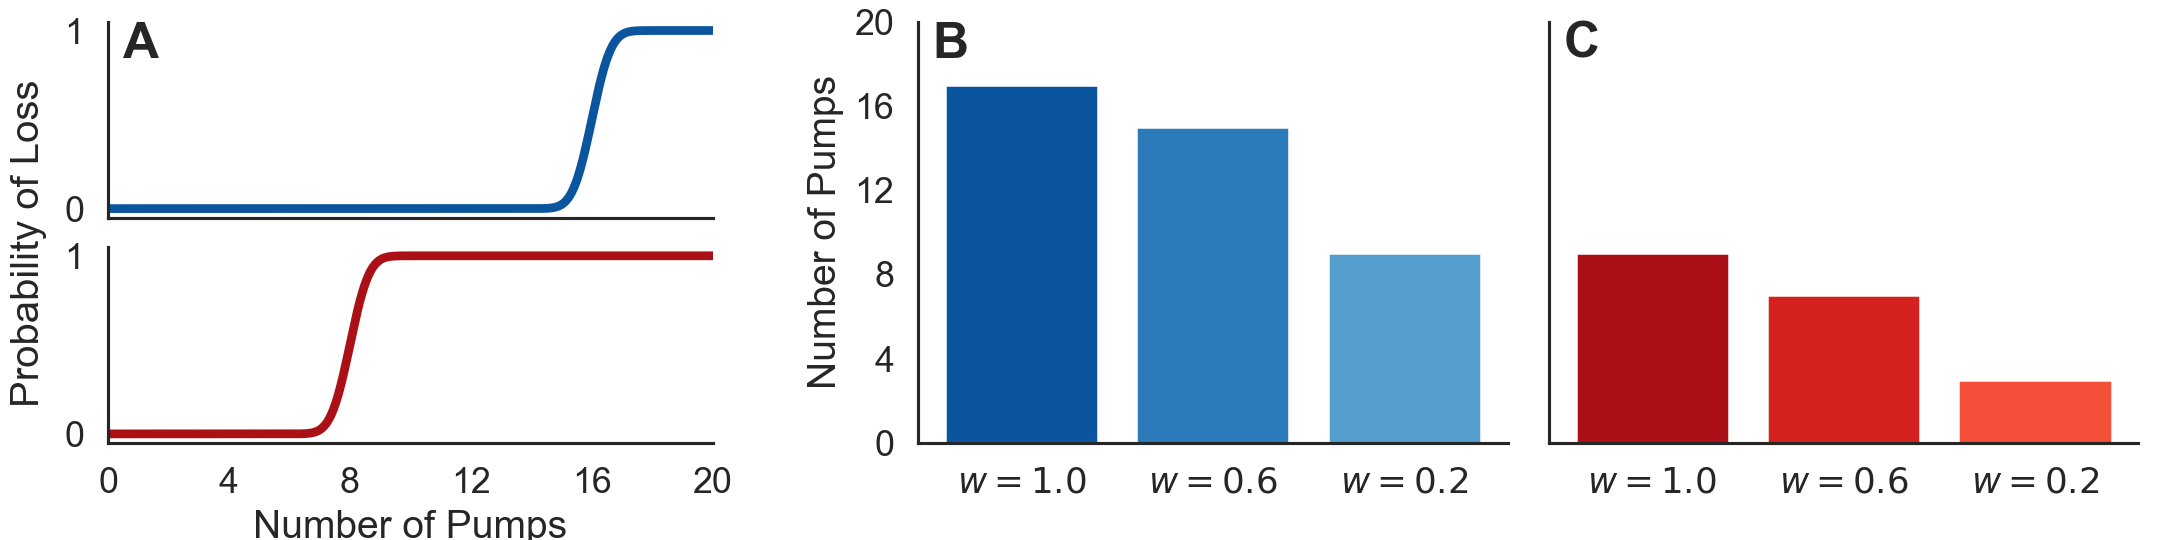
\includegraphics[trim={0 0 0 0},clip]{../figures/02_bart.png}}%
  }
  \par \textbf{Figure 2:} The Balloon Analog Risk Task (BART). The risk of balloon burst (point loss) increases with each pump (A). The optimal policy (number of pumps) under increasingly pessimistic learning is presented for low risk (B) and high risk (C) balloons. The optimistic agent ($w=1$) learns a policy reflecting the objective environmental risk. The moderate ($w=0.6$) and strongly ($w=0.2$) pessimistic agents learn to cash-out earlier, as is observed in anxious individuals. (Parameters: $\gamma = 1.0$)
\end{figure}

This empirical result is easily accounted for by our model. A simulation of performance on the BART is presented in Figure 2. For an optimistic agent ($w=1.0$), the optimal policy accurately reflects the statistics of the task. The optimal agent continues pumping the balloon until the marginal gain from one additional pump no longer exceeds the likelihood of of the balloon bursting. Thus, the optimistic agent continues pumping until reaching the (unobserved) mean number of pumps before the balloon bursts. The same is not true for the pessimistic agents. The moderately ($w=0.6$) and strongly ($w=0.2$) pessimistic agents exhibit behavioral policies with earlier cash-out times. The reason for this is that anticipated future harmful actions are able to exert influence on earlier states; risky pumps resulting in loss are more salient to these agents earlier in the trial. As such, the pessimistic agents perform similarly to what is observed empirically in anxious individuals.

It is worth noting that these results are similar to recent findings regarding flight initiation distance (FID) and anxiety \citep{Mobbs2018, Mobbs2019}. FID refers to a concept from behavioral ecology that measures the leaving time of a foraging animal at risk of predation. In the prototypical FID scenario, an animal can choose either to continue exploiting resources (i.e. accrue reward) or flee an approaching predator. Similar to the BART, the longer an animal chooses to exploit the greater reward and risk it experiences. In a recent study, \cite{Mobbs2019} investigated the relationship between sub-clinical levels of anxiety and leaving times during a virtual FID task involving both fast- and slow-acting predators. Interestingly, sub-clinical anxiety did not correlate with leaving times for fast predators, but was correlated with earlier leaving times for slow predators. (Sub-clinical anxiety also correlated with BOLD activity in brain structures including the ventral hippocampus, medial prefrontal cortex, amygdala and insula.) The authors use these results to support an argument distinguishing between "reactive" responses associated with immediate threat and "cognitive" responses associated with impending danger. Similar to the BART results, our model can readily account for the "cognitive"-type threat response reported in \cite{Mobbs2019}; importantly though, these findings suggest that our model may not be applicable to all types of threat processing, such as those with little reliance on future expectations (such as in immediate threat).

Similarly related are recent studies on behavioral inhibition, a behavioral style characterized by a temporal delay to initiate approach behavior associated with the development of anxiety disorders \citep{bach2015, khemka2017}. \cite{bach2015} argues that behaviorally inhibited responses (e.g. slowed reaction times under threat) reflect a normative Pavlovian heuristic, developed over evolutionary time, that is instrumental in surveying the environment, avoiding detection by predators, and possibly even waiting out nearby threat. Evidence for this heuristic comes from a sequential approach-avoidance conflict task, wherein a participant may choose to exit a safe zone to collect valuable tokens adjacent to a "sleeping" virtual predator. With each token collected, the probability of the predator "waking up", unbeknownst to the participant, increases. Similar to the BART, if the predator catches the participant, all tokens accrued during that trial are lost. Importantly, \cite{bach2015} (and later \cite{khemka2017}) find that response times for choosing to leave the safe zone increase as a function of predation threat, even though response times have no bearing on whether the predator "awakes", in line with the interpretation of behavioral inhibition as Pavlovian heuristic. 

Our model can offer an alternative interpretation. As observed above, one consequence of uncertainty about avoiding harmful future actions is that antecedent actions become associated with threat. In the context of the sequential approach-avoidance task, our pessimistic bias should therefore reduce the value of the choice to leave the safe zone to collect tokens, making it closer in value to the choice to stay and forego future point collection. Insofar that choices between similarly valued options result in prolonged response times by virtue of increased decision conflict, then we should predict that anxious individuals would exhibit, in addition to earlier leaving times, slower responses in sequential approach-avoidance task independent of a Pavlovian heuristic. Further work is necessary to disentangle these two interpretations. 

\subsection{Anxiety-to-Depression Transition}

As will become clear, the previous section concerning approach-avoidance conflict is a natural interlude to discussing the relationship between anxiety and depression. Anxiety and depression are highly comorbid, with roughly 45\% of individuals with a lifetime depression diagnosis also diagnosed with at least one anxiety disorder \citep{kessler2015}. Because of their frequent co-occurrence, many clinical theories treat anxiety and depressive disorders as variant manifestations of the same latent mechanisms causing disruption to negative affective processes (for review, see \cite{jacobson2014}). Where the two families of disorders can be distinguished is in their relation to positive affect and reward processing. Some have argued that whereas both anxiety and depression both involve exaggerated threat appraisals and pessimistic future expectations, only depression involves the certain belief about the absence of future rewards. 

\begin{figure}
  \centerline{%
    \resizebox{1.0\textwidth}{!}{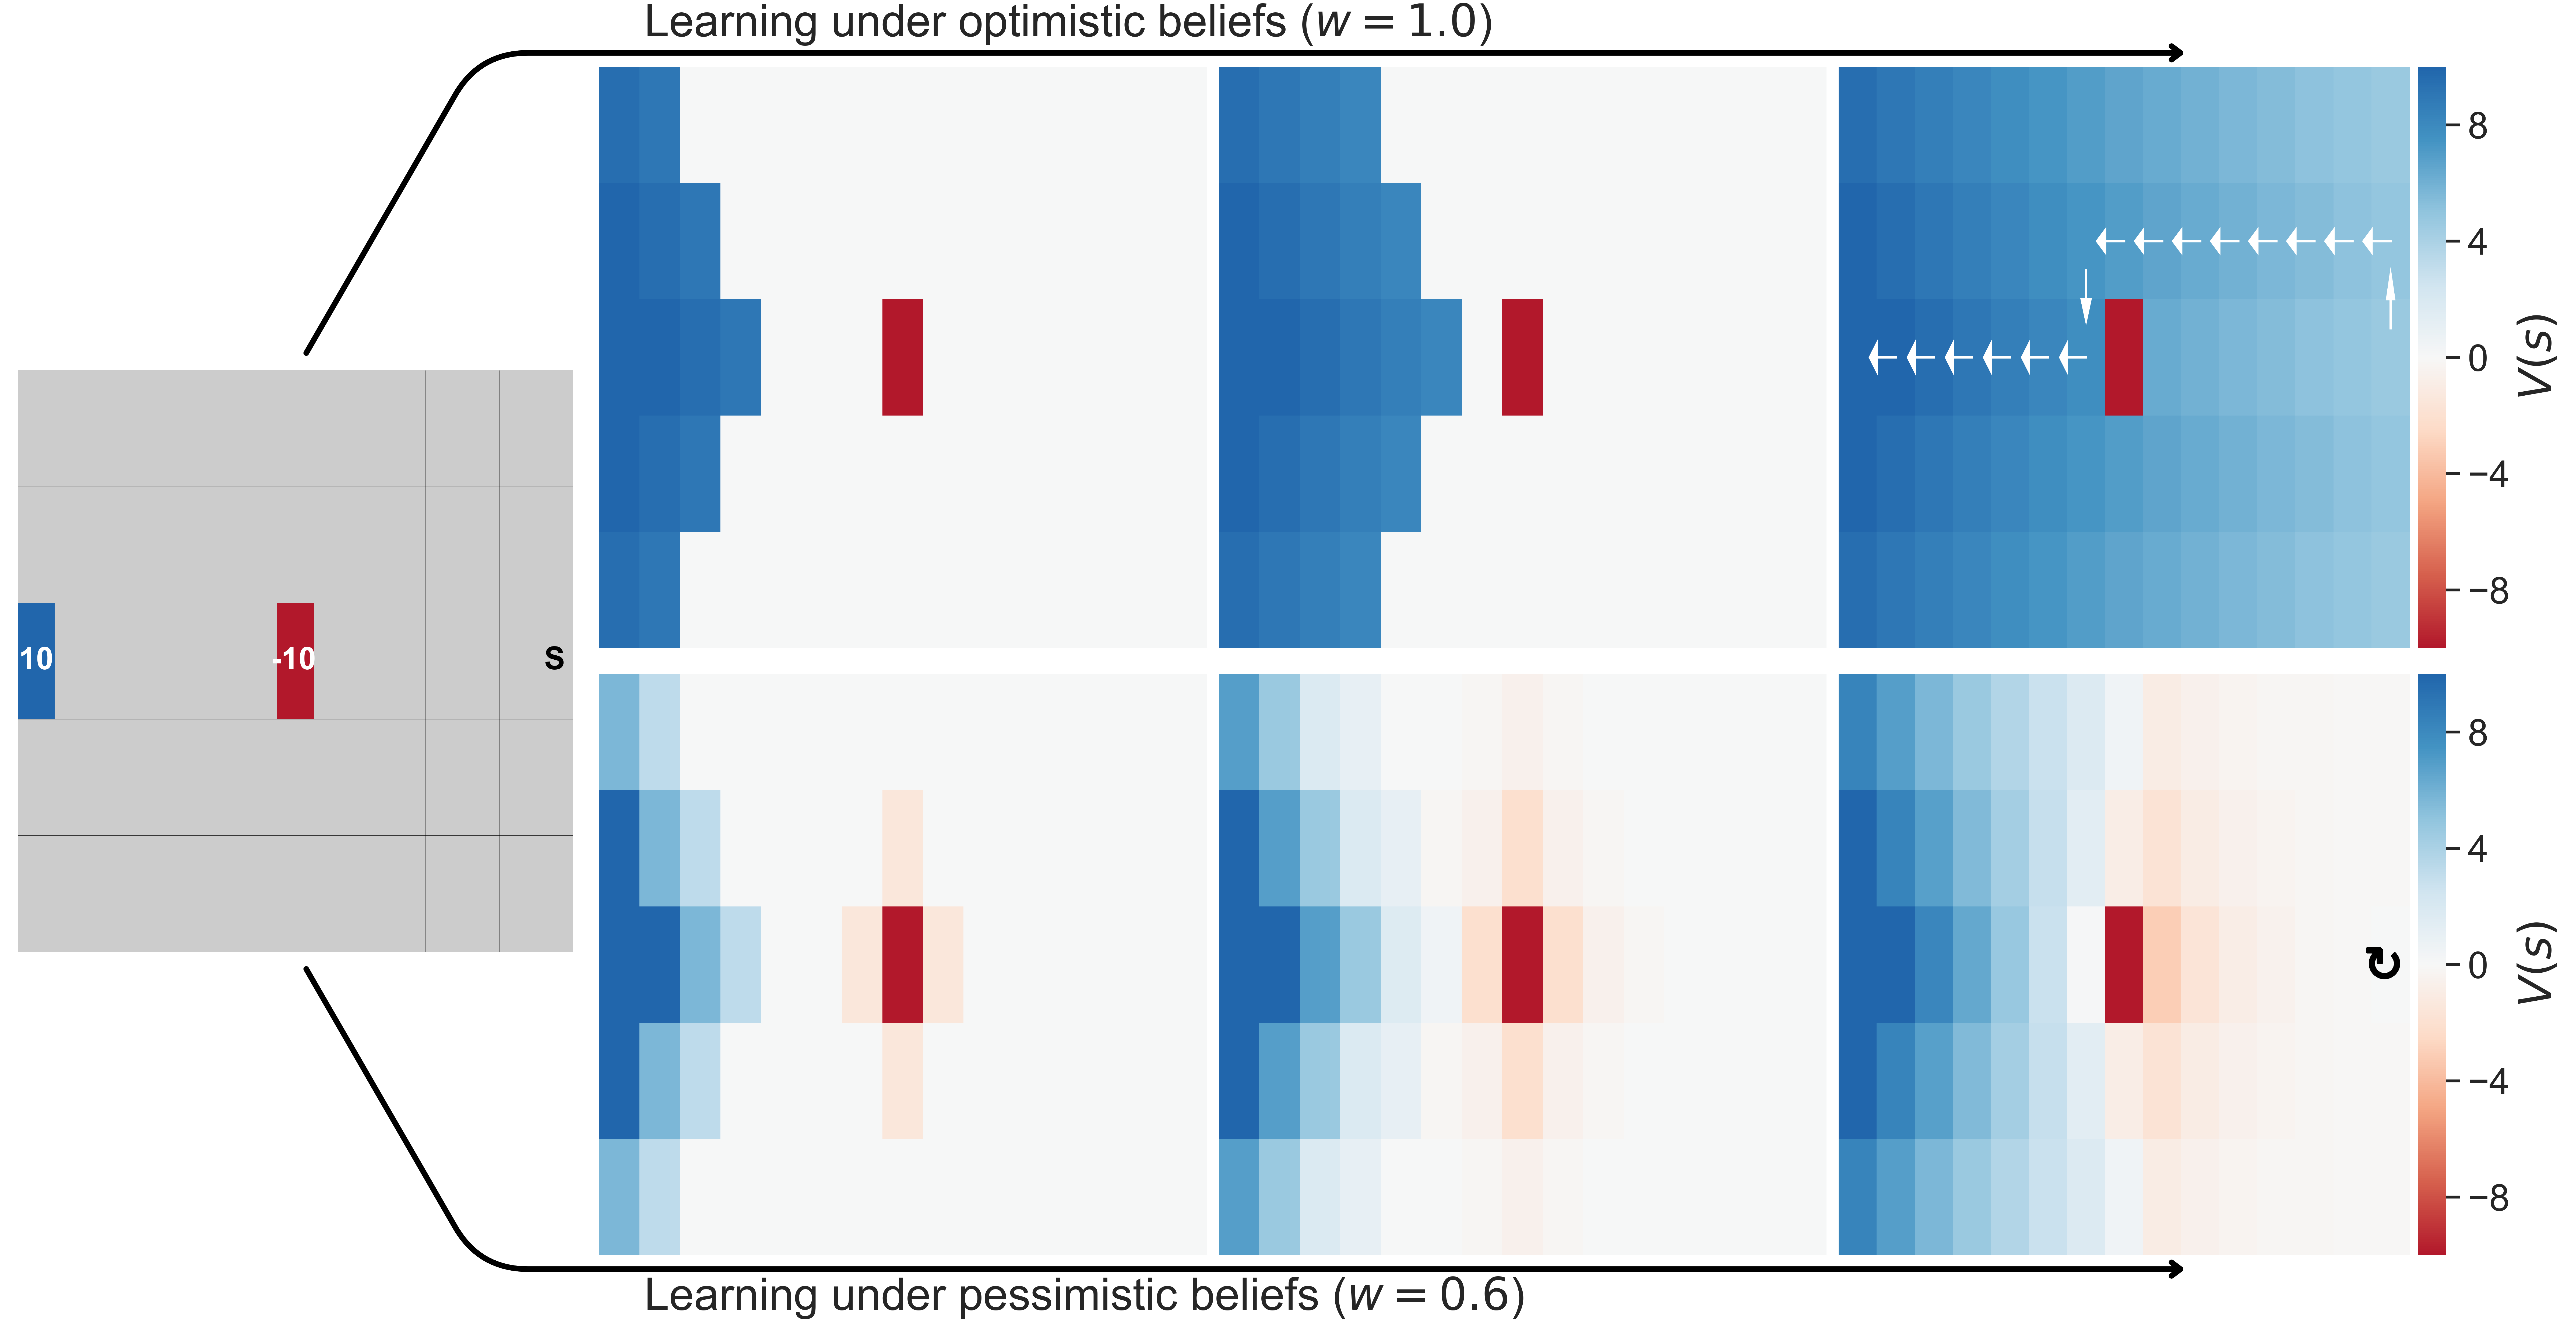
\includegraphics[trim={0 0 0 0},clip]{../figures/03_lh.png}}%
  }
  \par \textbf{Figure 3:} Progression from anxiety to depression. In this open environment, an agent starts opposite a reward (blue) with harm separating them (A). For an optimistic agent ($w=1$), positive value spreads from the reward to the starting tile (Panels B-D, left-to-right). Harm is mitigated through the belief of future self-efficacy. For a pessimistic agent ($w=0.6$), both positive and negative value spread (Panels E-G, left-to-right). Given the agent's closer proximity to harm than reward, the optimal policy for this agent is to stay at the initial state. (Parameters: $\gamma = 0.95$)
\end{figure}

One interesting proposal in the clinical literature attempting to explain this divergence appeals to longitudinal association between anxiety disorders and depression. Specifically, it has been proposed that the onset of at least certain types of anhedonic depression are preceded first by the onset of an anxiety disorder \citep{alloy1990, moitra2008, jacobson2014}. The idea according to this view is that because anxiety is associated with a bias towards avoidance behavior, then anxious individuals should be more likely to forego reward and other positive events in their everyday lives. Over time, it is argued, this should translate to a stable belief that, in addition to threat being unavoidable, reward is unobtainable thereby resulting in reduced behavioral activation and increased motor inhibition. Recent large-scale epidemiological studies have provided some empirical support for this claim, finding that anxiety symptoms often precede depression (\cite{mathew2011, jacobson2014, kessler2015}; though also see \cite{jacobson2017, plana2019}). Interestingly, one study event found that anxious avoidance behaviors were predictive future depression onset over a decade later \citep{jacobson2014}.

Though currently speculative, this prediction is accommodated by our model. Simulations of how this might come about is presented in Figure 3. We assume an open grid world, similar to that presented in Figure 1, except that rewards and harms are now (spatially) correlated. Figure 3a shows that, in order to reach the reward, an agent must approach (but need not encounter) danger. As above, the world is deterministic such that the presence of the harmful state poses no objective danger to the agent. The learning progression of an optimistic agent ($w=1$) reflects this (Figure 3b-d). An optimistic agent believes it will be able to act in accordance to its reward-maximizing preferences in the future; as such, it does not worry that it may inadvertently encounter danger in the future. As a consequence, only reward opportunity propagates from the source to its antecedent states whereas harm is effectively sequestered. The optimistic agent thereby learns a path from the start to reward in spite of the presence of a dangerous state.

In contrast, a pessimistic agent ($w=0.6$) is uncertain about its ability to effectively avoid future danger. As a consequence, reward and threat values propagate from their respective sources to their antecedent states (Figure 3e-g). Because reward and threat are (spatially) correlated in this environment, however, subjective threat increases with proximity to reward. As such, the pessimistic agent learns a behavioral policy distinct from the optimistic agent. Whereas the optimistic agent learns a path which circumnavigates danger, the pessimistic agent learns that any step toward reward is also a step towards danger. Consequently, the pessimistic agent learns to not move. In effect, the pessimistic agent exhibits a form of motor inhibition and immobility like that observed in depression. Moreover, as a function of its learned behavioral policy, the agent should not expect reward from the environment. In summary, our model can accommodate previous clinical theories about the transition from anxiety to depression; specifically, our model predicts that when reward and danger are correlated, pessimistic expectations and anxious avoidance can result over time in depression-like motor inhibition.

\subsection{Planning \& Aversive Pruning}

In large sequential choice environments, the total number of possible choice sequences grows exponentially with sequence length. As such, it is infeasible (if not impossible) for an agent to exhaustively evaluate all possible sequences of choices in order to carry out the one which maximizes reward. It is plausible then that rational agents may develop useful heuristics for winnowing out likely sub-optimal choice sequences. One such heuristic that has been proposed is aversive pruning \citep{Huys2012}, which is characterized as a Pavlovian response to losses such that choice sequences involving large losses are discarded from further evaluation during planning. 

\cite{Huys2012} (and later \cite{Lally2017}) sought evidence for aversive pruning in the decision tree environment presented in Figure 4a. Participants in these experiments received extensive training in this environment such that participants reportedly knew well both the transition and reward structure of the tree. During testing, participants completed a number of free-planning trials in which participants started at various states within the tree and selected paths along the tree so as to maximize reward. \cite{Huys2012} and \cite{Lally2017} predicted that participants starting at the top of the tree (as depicted in Figure 4a) would be more likely to discard the left branch as it involved an immediate large loss and would likely be discarded through aversive pruning (and despite the fact that it was the parent path to the reward-maximizing choice sequence). Both \cite{Huys2012} and \cite{Lally2017} reported that many participants exhibited this pattern of behavior in evidence of an aversive pruning heuristic. Most importantly for present purposes, \cite{Huys2012} and \cite{Lally2017} found the degree of aversive pruning was correlated with depressive and anxiety symptoms, respectively.

\begin{figure}
  \centerline{%
    \resizebox{1.0\textwidth}{!}{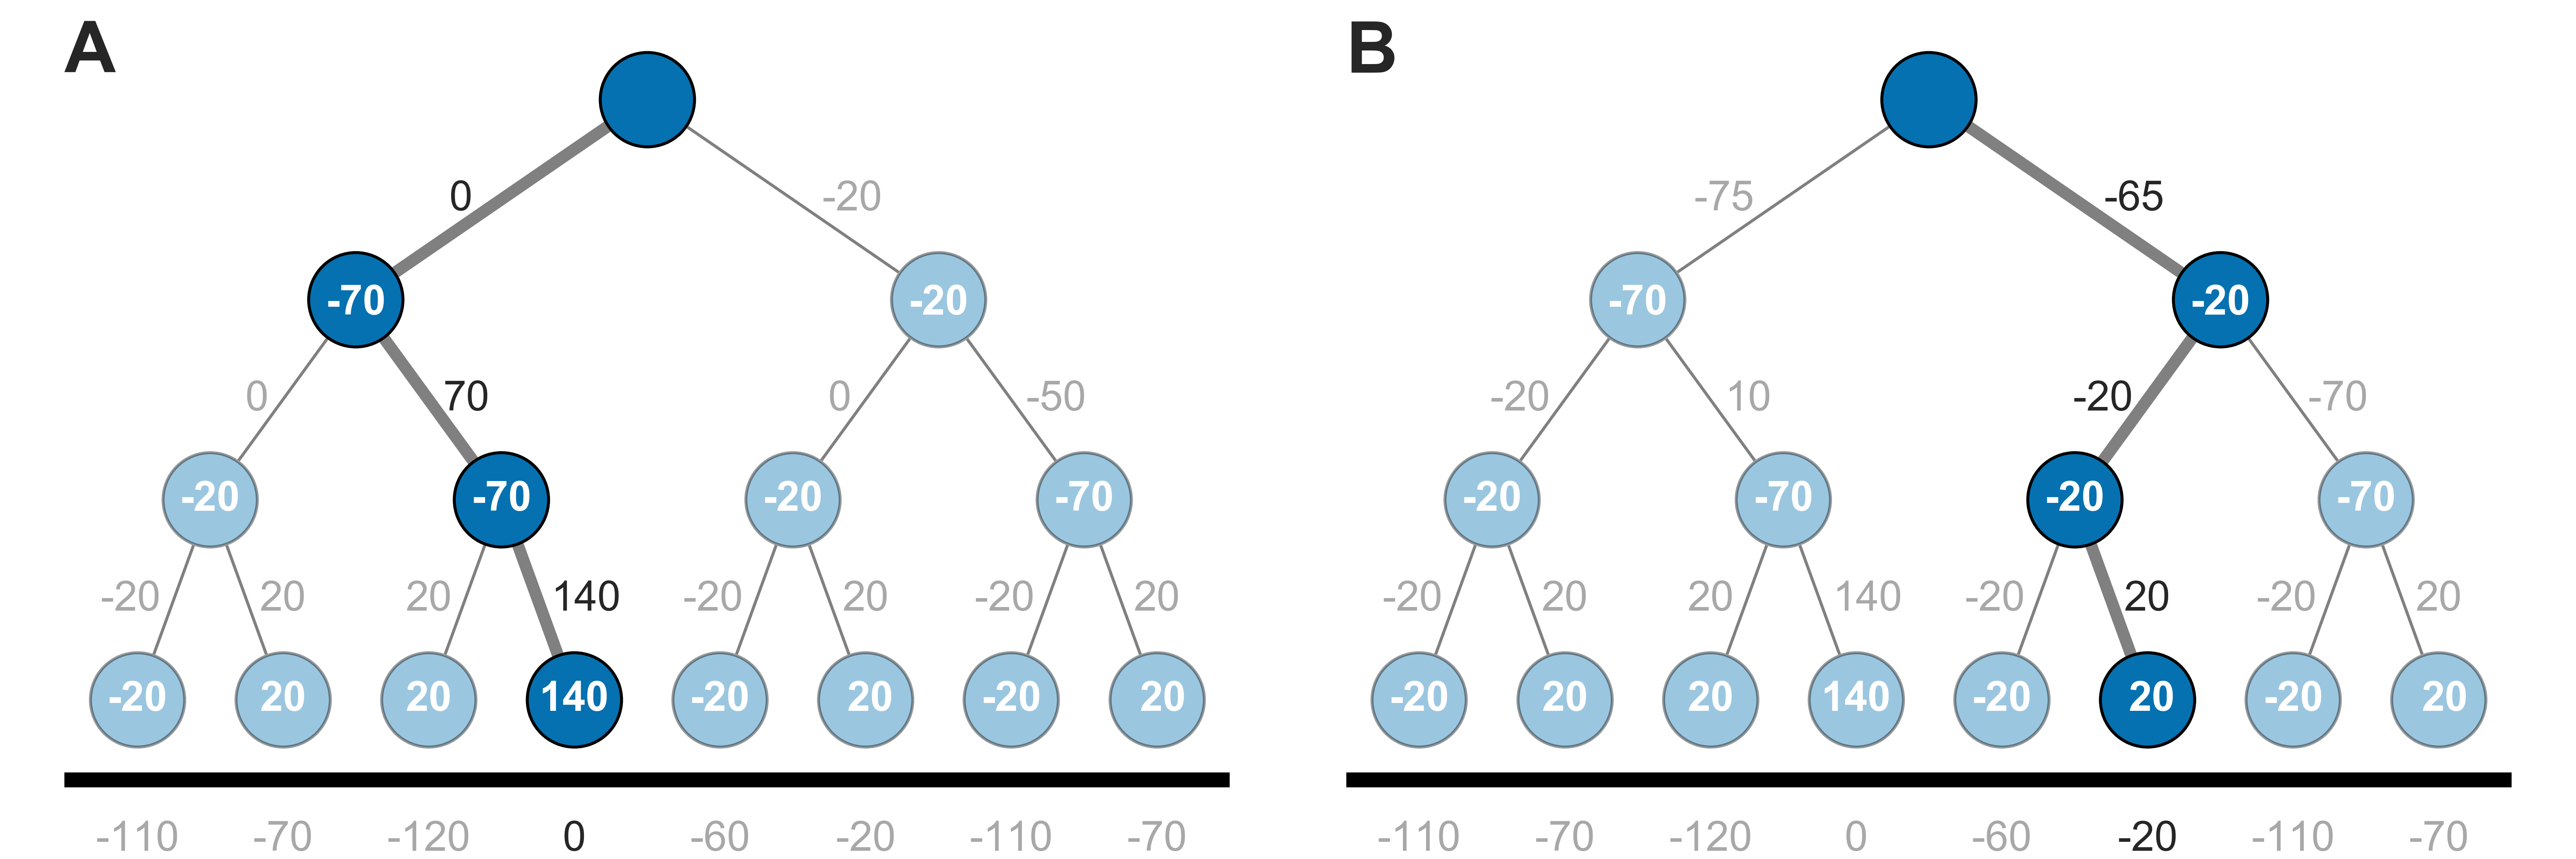
\includegraphics[trim={0 0 0 0},clip]{../figures/04_tree.png}}%
  }
  \par \textbf{Figure 4:} The decision tree environment from \cite{Huys2012} and \cite{Lally2017} (A). An optimistic agent ($w=1$) learns the optimal loss-minimizing policy through the initial large loss (B). A moderately pessimistic agent ($w=0.75$) will find both arms equally preferable insofar that it is less confident it will be able to execute optimal future choices (C). More pessimistic agents comes to prefer the branch without the large loss so as to avoid being unable to recoup the large initial loss (D).
\end{figure}

The aversive pruning heuristic is an intuitive and sensible strategy for circumventing exhaustive search, which draws upon a rich literature of Pavlovian biases. We note, however, that our model makes similar predictions in the decision tree environment employed by \cite{Huys2012} and \cite{Lally2017}. Assuming exhaustive training, the optimal policy for an optimistic agent ($w=1.0$) beginning at the top of the tree is presented in Figure 4b. Note the optimistic agent traverses through the initial large loss in order to complete the sequence that maximizes reward (minimizes loss). Different patterns of behavior are exhibited by moderate ($w=0.75$, Figure 4c) and strongly ($w=0.50$, Figure 4d) pessimistic agents. For these agents, the possibility of inadvertently choosing a future sub-optimal path, and accruing a large loss, are non-negligible. As such, preference for the objectively sub-optimal path not involving the large loss becomes increasingly preferred. This preference is reminiscent of what is observed for the subclinically depressed and anxious participants in the original studies, suggesting that our model may also describe anxious decision making in this task. This is not implausible insofar that working memory ability is often impaired in anxiety disorders \citep{Moran2016}, and pessimistic expectations about future choice may be warranted as such. 

We note that this reinterpretation of results is not meant to replace the aversive pruning heuristic. Our model makes no strong claims about mechanistic interpretations, and thus does not address the issue of computational intractability whereas the aversive pruning heuristic does. We are simply noting that they make similar behavior predictions for anxious decision making in the decision tree environment used thus far. Interestingly, these accounts could be disentangled through a minor manipulation of the choice environment presented above. One would simply need to move the large loss to later in the tree. Under the aversive pruning view, large losses only impact choice behavior when encountered in sequence. Under pessimistic sequential choice inference, however, future large losses impact antecedent states, making their selection less likely. Thus, a slight modification to the decision tree structure presented in Figure 4a might be used to disentangle which of the two theories better accounts for anxious decision making in the task.

\subsection{Free Choice Premium}

In this final section, we offer a novel prediction regarding the free choice premium. If an agent assumes they will be able to act in accordance to their (reward-maximizing) preferences in the future, then it follows that choices that enable an individual to make a future choice should be preferable to situations in which an individual is not. At worst, an agent is no better off than if they had not made a choice; at best, an agent is better able to steer themselves towards a desired outcome. Such is the logic that underlies an emerging literature suggesting that choice is inherently valuable \citep{Leotti2010}.

A free choice premium (i.e. choice is inherently valuable, all else being equal) has been observed across several behavioral experiments \citep{Suzuki1997, Leotti2011, Leotti2014, Cockburn2014} using several different experimental protocols. For present purposes, we will describe the protocol used by \cite{Leotti2011, Leotti2014}. Here, participants complete a two-stage decision making task (Figure 5a). In the first stage, participants choose between two cues: one yielding a future free choice and the other yielding a future fixed choice. In the second stage, participants either make a second choice (free choice) or have a choice made for them (fixed choice). Unbeknownst to participants, all choices in the second stage yield a reward drawn identical reward distributions; thus, no choice is actually advantageous in the long-run. The free choice premium is measured as a preference for the cue leading to free choice. \cite{Leotti2011, Leotti2014} find that participants prefer the cue leading to future choice, despite this conferring no objective benefit to participants.

We hypothesize that the free choice premium is contingent on an agent's positive expectations about its future actions. If this is true, it stands to reason that the free choice premium should be absent in anxious individuals. We present simulations of this effect in Figure 5b using a virtual experiment similar to that used in \cite{Leotti2011, Leotti2014}. As expected, optimistic agents ($w=1.0$) exhibit the free choice premium, measured as a preference for the cue leading to future choice. In contrast, moderately ($w=0.5$) and strongly ($w=0.0$) pessimistic agents exhibit a diminished free choice bias. In these agents, the value of worst action in the free choice is able to propagate backwards to the free choice action in stage 1. As such, the free choice confers no subjective benefit to the simulated agents and thus the free choice premium disappears. We plan on explicitly testing this hypothesis in subclinical and clinical anxiety in the near future.

\begin{figure}
  \centerline{%
    \resizebox{1.0\textwidth}{!}{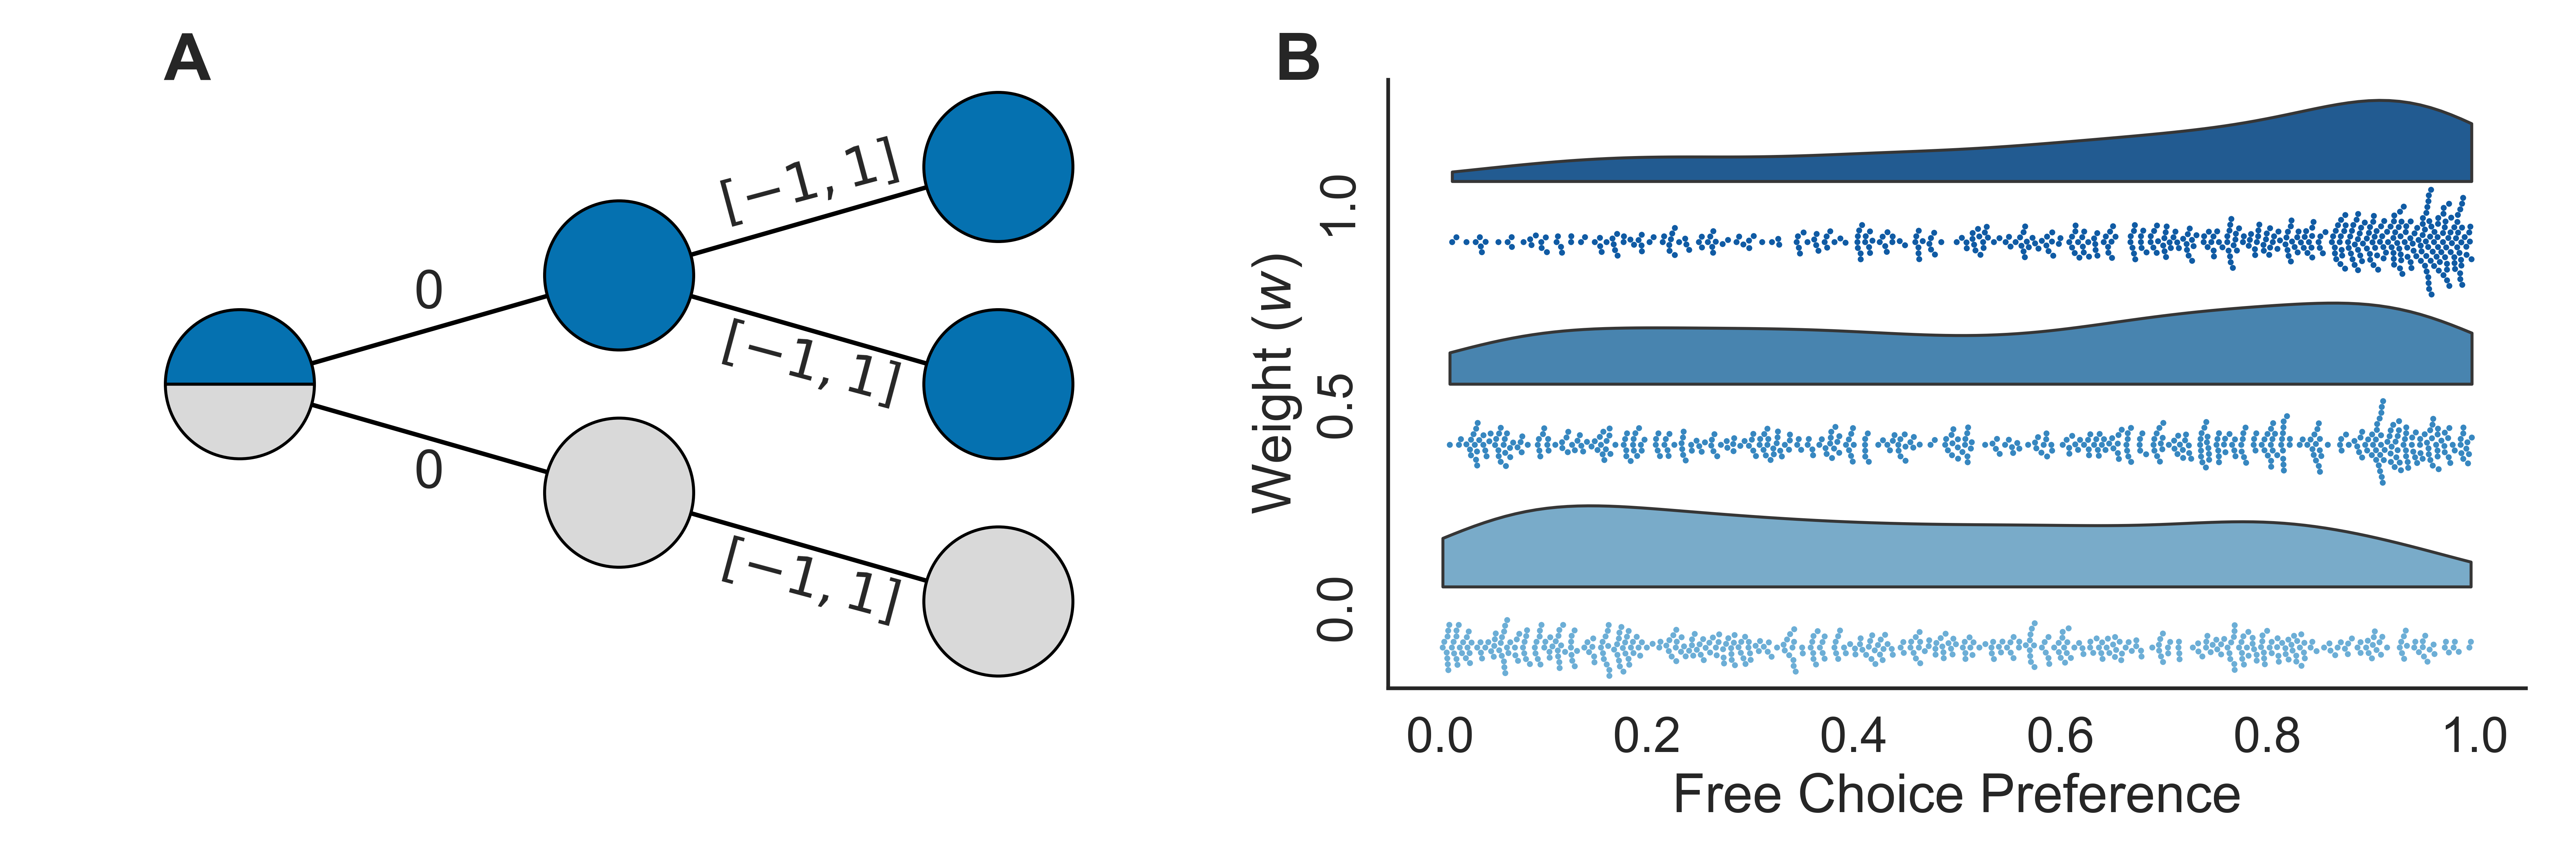
\includegraphics[trim={0 0 0 0},clip]{../figures/05_choice.png}}%
  }
  \par \textbf{Figure 5:} Schematic of the free choice bias tasks used in \cite{Leotti2011, Leotti2014} (A). The free choice bias is diminished in increasingly pessimistic agents (B).
\end{figure}

\section{Discussion}

Central to the acquisition and maintenance of anxiety disorders are symptoms including pessimistic inference, second-order conditioning, and persistent avoidance. In this article, we presented a simple computational account of these aberrations in learning and decision making. Specifically, we showed how a loss of confidence in the reliability of the future self and/or the environment can effectively backpropagate negative value across states of the environment. The result of this process are a series of inferences and behaviors resembling those observed in clinical anxiety. Though this is by no means a complete account of anxiety, the present model helps to explain the core symptoms of anxiety under one unifying framework.

Importantly, this computational account draws upon a longstanding recognition of the importance of perceived control to the development and maintenance of anxiety disorders. Central to many prominent theories of anxiety in the clinical literature highlight is a perceived lack of control. For example, learned helplessness theory and its successors claim that pathological anxiety results from a stable belief that the environment is uncontrollable, such that threat cannot be effectively mitigated. In contrast, Bandura's self-efficacy theory of anxiety posited that a lack of confidence in one's own ability to effectively handle threat was central to the pathogenesis of anxiety. Later theories, such as the triple vulnerability model, are equivocal as to whether an unreliable future environment or self is the root cause of anxiety, but highlights control beliefs as being a necessary compontent for developing anxiety. As we note above, the present model can accommodate either effect. Insofar that the state transition function and future state-action function are multiplicative, a pessimistic change to either should make similar predictions. It is possible that under certain conditions they may predict different outcomes. Future work may tease these apart, as they may be interesting for guiding treatment.

It is worth noting that we are not the first to attempt to formalize a theory of control in MDP. \cite{HuysDayan2009} provided a first computational account of learned helplessness through simple models of action-outcome contingencies. \cite{HuysDayan2009} found that training an agent first in an unreliable environment led to later impaired learning, akin to early learned helplessness experiments, by virtue of the prior of controllability. This provides a nice demonstration of learning impairment of action-outcome contingencies. Importantly, our accounts differ in at least three respects. First, we consider sequential decision environments, which is necessary for more accurately characterizing the symptoms of anxiety disorders. Second, our account specifies a mechanism by which the worst outcomes are realized; in their account, the world simply becomes random. This pessimism seems closer to what is observed in anxiety disorders. Finally, our account accounts for the persistence of these symptoms. Presumably, their model would eventually learn to escape with additional training; our account shows aberrant behaviors in the optimal (long-run) policy.

In this article, we discussed two mechanisms by which negative values can spread, through the state transition distribution and future state-action action. There is a third that we did not address here: that of the state itself. Here we assumed that states were fully observable; in other words, there was no uncertainty about the state an agent was currently occupying. In partially-observable Markov decision problems, the state itself must be inferred from external and internal variables. This is yet another means by which bad value can spread if undue likelihood is granted to undesirable or aversive states. This ideas has previously been proposed to explain some symptoms in anxiety \citep{Paulus2012}, and not without good reason. Anxiety disorders involve negatively biased interpretation of ambiguous percepts \citep{Hartley2012}, which may result in aberrant planning and increased avoidance for similar reasons to those described above. This is an area for future research.

In this article, we have explored a computational principle of approach and avoidance learning in sequential decision environments. We have not discussed, however, the particular psychological or neurobiological mechanisms by which this sort of learning may take place. This issue has been discussed in detail elsewhere \citep{Bishop2018}, but we briefly discuss a few possibilities here. One possibility is in biased sampling. If decision making and planning may rely on internal sampling from previously experienced episodes in order to make predictions about future value, then biased sampling may result in maladaptive decision making. Recent work has shown how finite sampling during planning can result in risk aversion and the overrepresentation of low probability but strongly negative outcomes (Lieder et al., 2018). Such a mechanism is prima facie in line with results showing the availability in memory of negative outcomes being higher for patients with anxiety \citep{Borkovec1999, Miranda2007}. Another possibility are an overreliance on Pavlovian heuristics, such as aversive pruning \citep{Huys2012,Lally2017}. As discussed above, future work should tease apart the predictions of our model and the aversive pruning heuristic.

Several recent studies have found evidence suggesting increased learning rates for negative reward prediction errors in individuals with elevated levels of anxiety \citep{Harle2017, Garrett2018, Aylward2019}. Though incearned learning from negative reward prediction errors may result in anxiety-like behaviors, these are likely not the sole cause of anxiety disorders for the reasons discussed above. Future research might investigate the relationship of prior beliefs about the reward statistics of the environment and learning to positive and negative prediction errors. A separate interestisng possibility is prioritized replay (Russek et al., 2017; Mattar and Daw, 2018). Offline replay of previous experiences (through hippocampal mechanisms) are known to facilitate learning. It has been proposed that biased replay could bias value estimates (Gagne et al., 2018).

\bibliographystyle{vancouver-authoryear}
\bibliography{citations}

\end{document}
